\documentclass[1p]{elsarticle_modified}
%\bibliographystyle{elsarticle-num}

%\usepackage[colorlinks]{hyperref}
%\usepackage{abbrmath_seonhwa} %\Abb, \Ascr, \Acal ,\Abf, \Afrak
\usepackage{amsfonts}
\usepackage{amssymb}
\usepackage{amsmath}
\usepackage{amsthm}
\usepackage{scalefnt}
\usepackage{amsbsy}
\usepackage{kotex}
\usepackage{caption}
\usepackage{subfig}
\usepackage{color}
\usepackage{graphicx}
\usepackage{xcolor} %% white, black, red, green, blue, cyan, magenta, yellow
\usepackage{float}
\usepackage{setspace}
\usepackage{hyperref}

\usepackage{tikz}
\usetikzlibrary{arrows}

\usepackage{multirow}
\usepackage{array} % fixed length table
\usepackage{hhline}

%%%%%%%%%%%%%%%%%%%%%
\makeatletter
\renewcommand*\env@matrix[1][\arraystretch]{%
	\edef\arraystretch{#1}%
	\hskip -\arraycolsep
	\let\@ifnextchar\new@ifnextchar
	\array{*\c@MaxMatrixCols c}}
\makeatother %https://tex.stackexchange.com/questions/14071/how-can-i-increase-the-line-spacing-in-a-matrix
%%%%%%%%%%%%%%%

\usepackage[normalem]{ulem}

\newcommand{\msout}[1]{\ifmmode\text{\sout{\ensuremath{#1}}}\else\sout{#1}\fi}
%SOURCE: \msout is \stkout macro in https://tex.stackexchange.com/questions/20609/strikeout-in-math-mode

\newcommand{\cancel}[1]{
	\ifmmode
	{\color{red}\msout{#1}}
	\else
	{\color{red}\sout{#1}}
	\fi
}

\newcommand{\add}[1]{
	{\color{blue}\uwave{#1}}
}

\newcommand{\replace}[2]{
	\ifmmode
	{\color{red}\msout{#1}}{\color{blue}\uwave{#2}}
	\else
	{\color{red}\sout{#1}}{\color{blue}\uwave{#2}}
	\fi
}

\newcommand{\Sol}{\mathcal{S}} %segment
\newcommand{\D}{D} %diagram
\newcommand{\A}{\mathcal{A}} %arc


%%%%%%%%%%%%%%%%%%%%%%%%%%%%%5 test

\def\sl{\operatorname{\textup{SL}}(2,\Cbb)}
\def\psl{\operatorname{\textup{PSL}}(2,\Cbb)}
\def\quan{\mkern 1mu \triangleright \mkern 1mu}

\theoremstyle{definition}
\newtheorem{thm}{Theorem}[section]
\newtheorem{prop}[thm]{Proposition}
\newtheorem{lem}[thm]{Lemma}
\newtheorem{ques}[thm]{Question}
\newtheorem{cor}[thm]{Corollary}
\newtheorem{defn}[thm]{Definition}
\newtheorem{exam}[thm]{Example}
\newtheorem{rmk}[thm]{Remark}
\newtheorem{alg}[thm]{Algorithm}

\newcommand{\I}{\sqrt{-1}}
\begin{document}

%\begin{frontmatter}
%
%\title{Boundary parabolic representations of knots up to 8 crossings}
%
%%% Group authors per affiliation:
%\author{Yunhi Cho} 
%\address{Department of Mathematics, University of Seoul, Seoul, Korea}
%\ead{yhcho@uos.ac.kr}
%
%
%\author{Seonhwa Kim} %\fnref{s_kim}}
%\address{Center for Geometry and Physics, Institute for Basic Science, Pohang, 37673, Korea}
%\ead{ryeona17@ibs.re.kr}
%
%\author{Hyuk Kim}
%\address{Department of Mathematical Sciences, Seoul National University, Seoul 08826, Korea}
%\ead{hyukkim@snu.ac.kr}
%
%\author{Seokbeom Yoon}
%\address{Department of Mathematical Sciences, Seoul National University, Seoul, 08826,  Korea}
%\ead{sbyoon15@snu.ac.kr}
%
%\begin{abstract}
%We find all boundary parabolic representation of knots up to 8 crossings.
%
%\end{abstract}
%\begin{keyword}
%    \MSC[2010] 57M25 
%\end{keyword}
%
%\end{frontmatter}

%\linenumbers
%\tableofcontents
%
\newcommand\colored[1]{\textcolor{white}{\rule[-0.35ex]{0.8em}{1.4ex}}\kern-0.8em\color{red} #1}%
%\newcommand\colored[1]{\textcolor{white}{ #1}\kern-2.17ex	\textcolor{white}{ #1}\kern-1.81ex	\textcolor{white}{ #1}\kern-2.15ex\color{red}#1	}

{\Large $\underline{11n_{3}~(K11n_{3})}$}

\setlength{\tabcolsep}{10pt}
\renewcommand{\arraystretch}{1.6}
\vspace{1cm}\begin{tabular}{m{100pt}>{\centering\arraybackslash}m{274pt}}
\multirow{5}{120pt}{
	\centering
	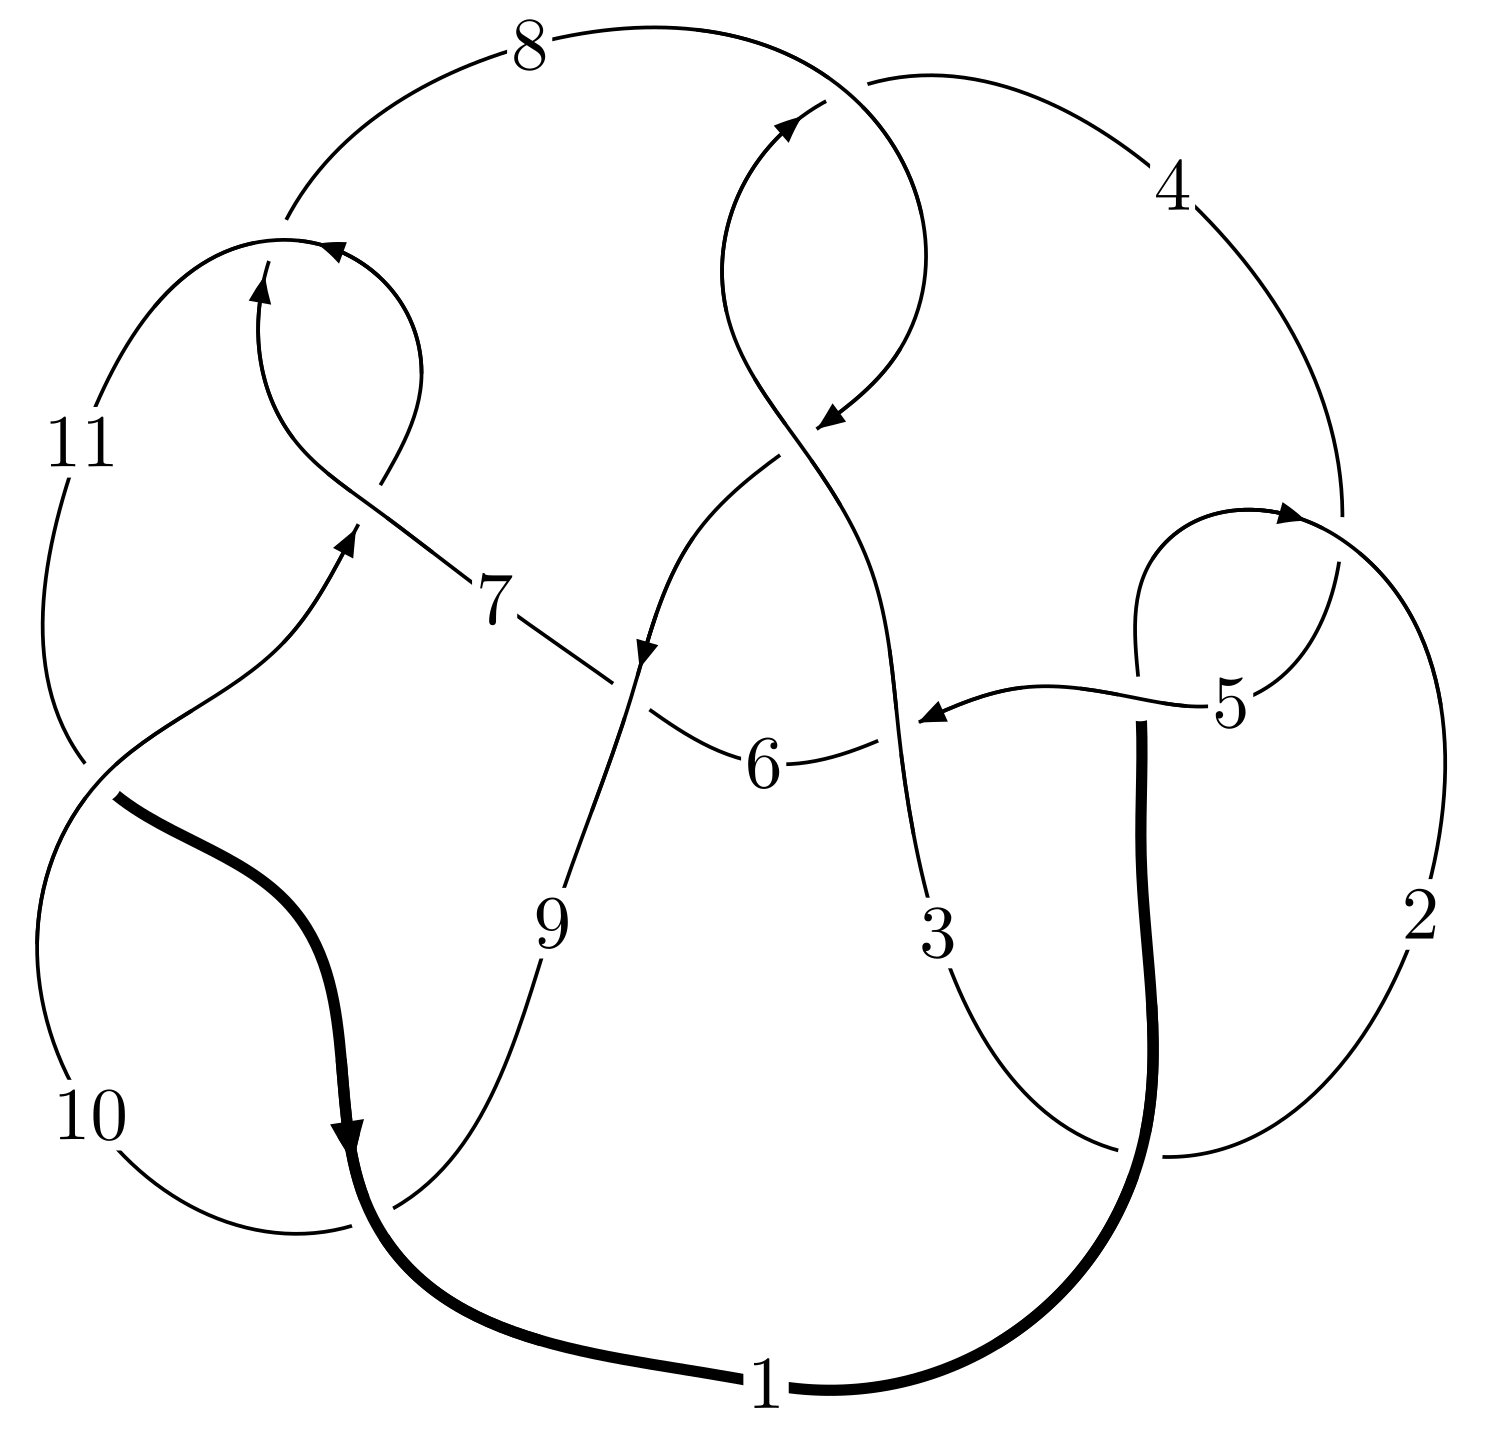
\includegraphics[width=112pt]{../../../GIT/diagram.site/Diagrams/png/619_11n_3.png}\\
\ \ \ A knot diagram\footnotemark}&
\allowdisplaybreaks
\textbf{Linearized knot diagam} \\
\cline{2-2}
 &
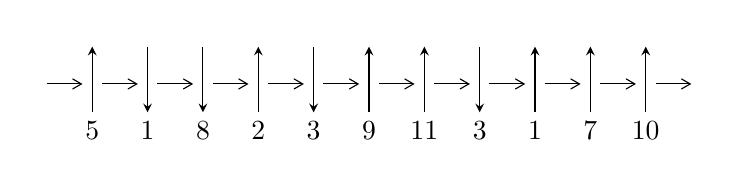
\begin{tikzpicture}[x=20pt, y=17pt]
	% nodes
	\node (C0) at (0, 0) {};
	\node (C1) at (1, 0) {};
	\node (C1U) at (1, +1) {};
	\node (C1D) at (1, -1) {5};

	\node (C2) at (2, 0) {};
	\node (C2U) at (2, +1) {};
	\node (C2D) at (2, -1) {1};

	\node (C3) at (3, 0) {};
	\node (C3U) at (3, +1) {};
	\node (C3D) at (3, -1) {8};

	\node (C4) at (4, 0) {};
	\node (C4U) at (4, +1) {};
	\node (C4D) at (4, -1) {2};

	\node (C5) at (5, 0) {};
	\node (C5U) at (5, +1) {};
	\node (C5D) at (5, -1) {3};

	\node (C6) at (6, 0) {};
	\node (C6U) at (6, +1) {};
	\node (C6D) at (6, -1) {9};

	\node (C7) at (7, 0) {};
	\node (C7U) at (7, +1) {};
	\node (C7D) at (7, -1) {11};

	\node (C8) at (8, 0) {};
	\node (C8U) at (8, +1) {};
	\node (C8D) at (8, -1) {3};

	\node (C9) at (9, 0) {};
	\node (C9U) at (9, +1) {};
	\node (C9D) at (9, -1) {1};

	\node (C10) at (10, 0) {};
	\node (C10U) at (10, +1) {};
	\node (C10D) at (10, -1) {7};

	\node (C11) at (11, 0) {};
	\node (C11U) at (11, +1) {};
	\node (C11D) at (11, -1) {10};
	\node (C12) at (12, 0) {};

	% arrows
	\draw[->,>={angle 60}]
	(C0) edge (C1) (C1) edge (C2) (C2) edge (C3) (C3) edge (C4) (C4) edge (C5) (C5) edge (C6) (C6) edge (C7) (C7) edge (C8) (C8) edge (C9) (C9) edge (C10) (C10) edge (C11) (C11) edge (C12) ;	\draw[->,>=stealth]
	(C1D) edge (C1U) (C2U) edge (C2D) (C3U) edge (C3D) (C4D) edge (C4U) (C5U) edge (C5D) (C6D) edge (C6U) (C7D) edge (C7U) (C8U) edge (C8D) (C9D) edge (C9U) (C10D) edge (C10U) (C11D) edge (C11U) ;
	\end{tikzpicture} \\
\hhline{~~} \\& 
\textbf{Solving Sequence} \\ \cline{2-2} 
 &
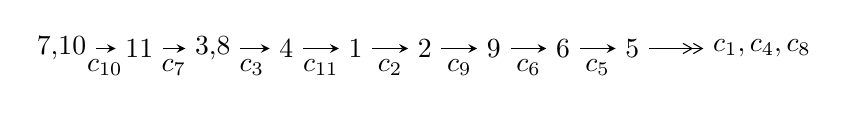
\begin{tikzpicture}[x=25pt, y=7pt]
	% node
	\node (A0) at (-1/8, 0) {7,10};
	\node (A1) at (1, 0) {11};
	\node (A2) at (33/16, 0) {3,8};
	\node (A3) at (25/8, 0) {4};
	\node (A4) at (33/8, 0) {1};
	\node (A5) at (41/8, 0) {2};
	\node (A6) at (49/8, 0) {9};
	\node (A7) at (57/8, 0) {6};
	\node (A8) at (65/8, 0) {5};
	\node (C1) at (1/2, -1) {$c_{10}$};
	\node (C2) at (3/2, -1) {$c_{7}$};
	\node (C3) at (21/8, -1) {$c_{3}$};
	\node (C4) at (29/8, -1) {$c_{11}$};
	\node (C5) at (37/8, -1) {$c_{2}$};
	\node (C6) at (45/8, -1) {$c_{9}$};
	\node (C7) at (53/8, -1) {$c_{6}$};
	\node (C8) at (61/8, -1) {$c_{5}$};
	\node (A9) at (10, 0) {$c_{1},c_{4},c_{8}$};

	% edge
	\draw[->,>=stealth]	
	(A0) edge (A1) (A1) edge (A2) (A2) edge (A3) (A3) edge (A4) (A4) edge (A5) (A5) edge (A6) (A6) edge (A7) (A7) edge (A8) ;
	\draw[->>,>={angle 60}]	
	(A8) edge (A9);
\end{tikzpicture} \\ 

\end{tabular} \\

\footnotetext{
The image of knot diagram is generated by the software ``\textbf{Draw programme}" developed by Andrew Bartholomew(\url{http://www.layer8.co.uk/maths/draw/index.htm\#Running-draw}), where we modified some parts for our purpose(\url{https://github.com/CATsTAILs/LinksPainter}).
}\phantom \\ \newline 
\centering \textbf{Ideals for irreducible components\footnotemark of $X_{\text{par}}$} 
 
\begin{align*}
I^u_{1}&=\langle 
-5 u^{26}+11 u^{25}+\cdots+2 b-5,\;u^{25}-2 u^{24}+\cdots+2 a+5 u,\;u^{27}-3 u^{26}+\cdots+3 u-1\rangle \\
I^u_{2}&=\langle 
u^2 a+b- a,\;- u^2 a+a^2- a u+u+1,\;u^3+u^2-1\rangle \\
\\
\end{align*}
\raggedright * 2 irreducible components of $\dim_{\mathbb{C}}=0$, with total 33 representations.\\
\footnotetext{All coefficients of polynomials are rational numbers. But the coefficients are sometimes approximated in decimal forms when there is not enough margin.}
\newpage
\renewcommand{\arraystretch}{1}
\centering \section*{I. $I^u_{1}= \langle -5 u^{26}+11 u^{25}+\cdots+2 b-5,\;u^{25}-2 u^{24}+\cdots+2 a+5 u,\;u^{27}-3 u^{26}+\cdots+3 u-1 \rangle$}
\flushleft \textbf{(i) Arc colorings}\\
\begin{tabular}{m{7pt} m{180pt} m{7pt} m{180pt} }
\flushright $a_{7}=$&$\begin{pmatrix}0\\u\end{pmatrix}$ \\
\flushright $a_{10}=$&$\begin{pmatrix}1\\0\end{pmatrix}$ \\
\flushright $a_{11}=$&$\begin{pmatrix}1\\- u^2\end{pmatrix}$ \\
\flushright $a_{3}=$&$\begin{pmatrix}-\frac{1}{2} u^{25}+u^{24}+\cdots+\frac{15}{2} u^2-\frac{5}{2} u\\\frac{5}{2} u^{26}-\frac{11}{2} u^{25}+\cdots-5 u+\frac{5}{2}\end{pmatrix}$ \\
\flushright $a_{8}=$&$\begin{pmatrix}u\\- u^3+u\end{pmatrix}$ \\
\flushright $a_{4}=$&$\begin{pmatrix}- u^{26}+\frac{5}{2} u^{25}+\cdots+\frac{3}{2} u-2\\\frac{1}{2} u^{26}-\frac{3}{2} u^{25}+\cdots+5 u^2+\frac{1}{2}\end{pmatrix}$ \\
\flushright $a_{1}=$&$\begin{pmatrix}- u^2+1\\- u^2\end{pmatrix}$ \\
\flushright $a_{2}=$&$\begin{pmatrix}- u^{25}+\frac{3}{2} u^{24}+\cdots-\frac{3}{2} u-\frac{1}{2}\\2 u^{26}-5 u^{25}+\cdots-4 u+2\end{pmatrix}$ \\
\flushright $a_{9}=$&$\begin{pmatrix}u^4- u^2+1\\u^4\end{pmatrix}$ \\
\flushright $a_{6}=$&$\begin{pmatrix}- u^9+2 u^7-3 u^5+2 u^3- u\\- u^9+u^7- u^5+u\end{pmatrix}$ \\
\flushright $a_{5}=$&$\begin{pmatrix}\frac{1}{2} u^{25}- u^{24}+\cdots+\frac{3}{2} u-1\\-\frac{1}{2} u^{26}+\frac{3}{2} u^{25}+\cdots+3 u-\frac{1}{2}\end{pmatrix}$\\ \flushright $a_{5}=$&$\begin{pmatrix}\frac{1}{2} u^{25}- u^{24}+\cdots+\frac{3}{2} u-1\\-\frac{1}{2} u^{26}+\frac{3}{2} u^{25}+\cdots+3 u-\frac{1}{2}\end{pmatrix}$\\&\end{tabular}
\flushleft \textbf{(ii) Obstruction class $= -1$}\\~\\
\flushleft \textbf{(iii) Cusp Shapes $= \frac{23}{2} u^{26}-24 u^{25}+\cdots-\frac{69}{2} u+\frac{25}{2}$}\\~\\
\newpage\renewcommand{\arraystretch}{1}
\flushleft \textbf{(iv) u-Polynomials at the component}\newline \\
\begin{tabular}{m{50pt}|m{274pt}}
Crossings & \hspace{64pt}u-Polynomials at each crossing \\
\hline $$\begin{aligned}c_{1},c_{4}\end{aligned}$$&$\begin{aligned}
&u^{27}+4 u^{26}+\cdots+4 u+1
\end{aligned}$\\
\hline $$\begin{aligned}c_{2}\end{aligned}$$&$\begin{aligned}
&u^{27}+6 u^{26}+\cdots+4 u-1
\end{aligned}$\\
\hline $$\begin{aligned}c_{3},c_{8}\end{aligned}$$&$\begin{aligned}
&u^{27}- u^{26}+\cdots-32 u-64
\end{aligned}$\\
\hline $$\begin{aligned}c_{5}\end{aligned}$$&$\begin{aligned}
&u^{27}-4 u^{26}+\cdots+6988 u+1153
\end{aligned}$\\
\hline $$\begin{aligned}c_{6}\end{aligned}$$&$\begin{aligned}
&u^{27}+3 u^{26}+\cdots- u-1
\end{aligned}$\\
\hline $$\begin{aligned}c_{7},c_{10}\end{aligned}$$&$\begin{aligned}
&u^{27}-3 u^{26}+\cdots+3 u-1
\end{aligned}$\\
\hline $$\begin{aligned}c_{9},c_{11}\end{aligned}$$&$\begin{aligned}
&u^{27}-11 u^{26}+\cdots-9 u-1
\end{aligned}$\\
\hline
\end{tabular}\\~\\
\newpage\renewcommand{\arraystretch}{1}
\flushleft \textbf{(v) Riley Polynomials at the component}\newline \\
\begin{tabular}{m{50pt}|m{274pt}}
Crossings & \hspace{64pt}Riley Polynomials at each crossing \\
\hline $$\begin{aligned}c_{1},c_{4}\end{aligned}$$&$\begin{aligned}
&y^{27}+6 y^{26}+\cdots+4 y-1
\end{aligned}$\\
\hline $$\begin{aligned}c_{2}\end{aligned}$$&$\begin{aligned}
&y^{27}+34 y^{26}+\cdots+136 y-1
\end{aligned}$\\
\hline $$\begin{aligned}c_{3},c_{8}\end{aligned}$$&$\begin{aligned}
&y^{27}+35 y^{26}+\cdots+1024 y-4096
\end{aligned}$\\
\hline $$\begin{aligned}c_{5}\end{aligned}$$&$\begin{aligned}
&y^{27}+62 y^{26}+\cdots-7660244 y-1329409
\end{aligned}$\\
\hline $$\begin{aligned}c_{6}\end{aligned}$$&$\begin{aligned}
&y^{27}-47 y^{26}+\cdots-9 y-1
\end{aligned}$\\
\hline $$\begin{aligned}c_{7},c_{10}\end{aligned}$$&$\begin{aligned}
&y^{27}-11 y^{26}+\cdots-9 y-1
\end{aligned}$\\
\hline $$\begin{aligned}c_{9},c_{11}\end{aligned}$$&$\begin{aligned}
&y^{27}+13 y^{26}+\cdots+127 y-1
\end{aligned}$\\
\hline
\end{tabular}\\~\\
\newpage\flushleft \textbf{(vi) Complex Volumes and Cusp Shapes}
$$\begin{array}{c|c|c}  
\text{Solutions to }I^u_{1}& \I (\text{vol} + \sqrt{-1}CS) & \text{Cusp shape}\\
 \hline 
\begin{aligned}
u &= \phantom{-}0.456584 + 0.907647 I \\
a &= -1.48477 - 0.61163 I \\
b &= -1.25986 + 0.88956 I\end{aligned}
 & \phantom{-}7.22245 + 1.02048 I & \phantom{-}3.69178 - 1.94630 I \\ \hline\begin{aligned}
u &= \phantom{-}0.456584 - 0.907647 I \\
a &= -1.48477 + 0.61163 I \\
b &= -1.25986 - 0.88956 I\end{aligned}
 & \phantom{-}7.22245 - 1.02048 I & \phantom{-}3.69178 + 1.94630 I \\ \hline\begin{aligned}
u &= \phantom{-}0.964922 + 0.396644 I \\
a &= -0.252553 + 0.564190 I \\
b &= \phantom{-}1.21469 + 1.07115 I\end{aligned}
 & \phantom{-}2.07980 + 1.34949 I & \phantom{-}7.85827 - 1.99966 I \\ \hline\begin{aligned}
u &= \phantom{-}0.964922 - 0.396644 I \\
a &= -0.252553 - 0.564190 I \\
b &= \phantom{-}1.21469 - 1.07115 I\end{aligned}
 & \phantom{-}2.07980 - 1.34949 I & \phantom{-}7.85827 + 1.99966 I \\ \hline\begin{aligned}
u &= \phantom{-}0.524863 + 0.914721 I \\
a &= \phantom{-}1.55069 + 0.62247 I \\
b &= \phantom{-}1.39313 - 0.99095 I\end{aligned}
 & \phantom{-}6.79111 - 5.64536 I & \phantom{-}3.12437 + 2.66728 I \\ \hline\begin{aligned}
u &= \phantom{-}0.524863 - 0.914721 I \\
a &= \phantom{-}1.55069 - 0.62247 I \\
b &= \phantom{-}1.39313 + 0.99095 I\end{aligned}
 & \phantom{-}6.79111 + 5.64536 I & \phantom{-}3.12437 - 2.66728 I \\ \hline\begin{aligned}
u &= -0.974186 + 0.462885 I \\
a &= \phantom{-}0.529071 - 0.939257 I \\
b &= \phantom{-}0.169302 - 0.547843 I\end{aligned}
 & \phantom{-}1.69325 - 4.38642 I & \phantom{-}5.48340 + 6.16823 I \\ \hline\begin{aligned}
u &= -0.974186 - 0.462885 I \\
a &= \phantom{-}0.529071 + 0.939257 I \\
b &= \phantom{-}0.169302 + 0.547843 I\end{aligned}
 & \phantom{-}1.69325 + 4.38642 I & \phantom{-}5.48340 - 6.16823 I \\ \hline\begin{aligned}
u &= -0.838777 + 0.356107 I \\
a &= -1.00459 + 1.02558 I \\
b &= -0.373891 + 0.589972 I\end{aligned}
 & \phantom{-}0.942185 + 1.033980 I & \phantom{-}3.86006 + 2.18156 I \\ \hline\begin{aligned}
u &= -0.838777 - 0.356107 I \\
a &= -1.00459 - 1.02558 I \\
b &= -0.373891 - 0.589972 I\end{aligned}
 & \phantom{-}0.942185 - 1.033980 I & \phantom{-}3.86006 - 2.18156 I\\
 \hline 
 \end{array}$$\newpage$$\begin{array}{c|c|c}  
\text{Solutions to }I^u_{1}& \I (\text{vol} + \sqrt{-1}CS) & \text{Cusp shape}\\
 \hline 
\begin{aligned}
u &= \phantom{-}0.685911 + 0.573005 I \\
a &= \phantom{-}1.282770 - 0.152453 I \\
b &= \phantom{-}0.13458 - 1.76175 I\end{aligned}
 & -1.54191 - 1.16661 I & \phantom{-}0.74423 + 1.49202 I \\ \hline\begin{aligned}
u &= \phantom{-}0.685911 - 0.573005 I \\
a &= \phantom{-}1.282770 + 0.152453 I \\
b &= \phantom{-}0.13458 + 1.76175 I\end{aligned}
 & -1.54191 + 1.16661 I & \phantom{-}0.74423 - 1.49202 I \\ \hline\begin{aligned}
u &= -0.821117 + 0.748475 I \\
a &= -0.420089 - 0.037335 I \\
b &= -0.229956 + 0.061310 I\end{aligned}
 & -3.44772 - 1.77523 I & -1.86458 + 4.75426 I \\ \hline\begin{aligned}
u &= -0.821117 - 0.748475 I \\
a &= -0.420089 + 0.037335 I \\
b &= -0.229956 - 0.061310 I\end{aligned}
 & -3.44772 + 1.77523 I & -1.86458 - 4.75426 I \\ \hline\begin{aligned}
u &= \phantom{-}0.960749 + 0.570989 I \\
a &= \phantom{-}0.404574 - 1.204920 I \\
b &= -1.74421 - 1.76576 I\end{aligned}
 & -0.68885 + 5.76088 I & \phantom{-}3.34925 - 6.52520 I \\ \hline\begin{aligned}
u &= \phantom{-}0.960749 - 0.570989 I \\
a &= \phantom{-}0.404574 + 1.204920 I \\
b &= -1.74421 + 1.76576 I\end{aligned}
 & -0.68885 - 5.76088 I & \phantom{-}3.34925 + 6.52520 I \\ \hline\begin{aligned}
u &= \phantom{-}0.866757\phantom{ +0.000000I} \\
a &= -0.0957077\phantom{ +0.000000I} \\
b &= \phantom{-}0.622584\phantom{ +0.000000I}\end{aligned}
 & \phantom{-}1.43125\phantom{ +0.000000I} & \phantom{-}6.84050\phantom{ +0.000000I} \\ \hline\begin{aligned}
u &= -0.922854 + 0.737156 I \\
a &= \phantom{-}0.035124 - 0.374638 I \\
b &= -0.045924 - 0.210874 I\end{aligned}
 & -3.14099 - 3.86941 I & \phantom{-}0.026459 + 0.626604 I \\ \hline\begin{aligned}
u &= -0.922854 - 0.737156 I \\
a &= \phantom{-}0.035124 + 0.374638 I \\
b &= -0.045924 + 0.210874 I\end{aligned}
 & -3.14099 + 3.86941 I & \phantom{-}0.026459 - 0.626604 I \\ \hline\begin{aligned}
u &= -1.242910 + 0.029552 I \\
a &= \phantom{-}0.02740 - 1.50043 I \\
b &= \phantom{-}0.006371 - 0.831742 I\end{aligned}
 & \phantom{-}13.47880 - 3.52700 I & \phantom{-}8.35802 + 2.34346 I\\
 \hline 
 \end{array}$$\newpage$$\begin{array}{c|c|c}  
\text{Solutions to }I^u_{1}& \I (\text{vol} + \sqrt{-1}CS) & \text{Cusp shape}\\
 \hline 
\begin{aligned}
u &= -1.242910 - 0.029552 I \\
a &= \phantom{-}0.02740 + 1.50043 I \\
b &= \phantom{-}0.006371 + 0.831742 I\end{aligned}
 & \phantom{-}13.47880 + 3.52700 I & \phantom{-}8.35802 - 2.34346 I \\ \hline\begin{aligned}
u &= \phantom{-}1.135150 + 0.655354 I \\
a &= \phantom{-}0.445958 + 1.202700 I \\
b &= \phantom{-}2.34089 + 0.91299 I\end{aligned}
 & \phantom{-}9.30444 + 4.72653 I & \phantom{-}5.93859 - 2.37138 I \\ \hline\begin{aligned}
u &= \phantom{-}1.135150 - 0.655354 I \\
a &= \phantom{-}0.445958 - 1.202700 I \\
b &= \phantom{-}2.34089 - 0.91299 I\end{aligned}
 & \phantom{-}9.30444 - 4.72653 I & \phantom{-}5.93859 + 2.37138 I \\ \hline\begin{aligned}
u &= \phantom{-}1.118230 + 0.692002 I \\
a &= -0.51886 - 1.31753 I \\
b &= -2.49328 - 0.90508 I\end{aligned}
 & \phantom{-}8.6132 + 11.5634 I & \phantom{-}4.87720 - 6.78953 I \\ \hline\begin{aligned}
u &= \phantom{-}1.118230 - 0.692002 I \\
a &= -0.51886 + 1.31753 I \\
b &= -2.49328 + 0.90508 I\end{aligned}
 & \phantom{-}8.6132 - 11.5634 I & \phantom{-}4.87720 + 6.78953 I \\ \hline\begin{aligned}
u &= \phantom{-}0.020052 + 0.347458 I \\
a &= -1.54687 - 0.86649 I \\
b &= -0.423137 + 0.416168 I\end{aligned}
 & -0.075638 + 1.377020 I & -0.36727 - 4.75192 I \\ \hline\begin{aligned}
u &= \phantom{-}0.020052 - 0.347458 I \\
a &= -1.54687 + 0.86649 I \\
b &= -0.423137 - 0.416168 I\end{aligned}
 & -0.075638 - 1.377020 I & -0.36727 + 4.75192 I\\
 \hline 
 \end{array}$$\newpage\newpage\renewcommand{\arraystretch}{1}
\centering \section*{II. $I^u_{2}= \langle u^2 a+b- a,\;- u^2 a+a^2- a u+u+1,\;u^3+u^2-1 \rangle$}
\flushleft \textbf{(i) Arc colorings}\\
\begin{tabular}{m{7pt} m{180pt} m{7pt} m{180pt} }
\flushright $a_{7}=$&$\begin{pmatrix}0\\u\end{pmatrix}$ \\
\flushright $a_{10}=$&$\begin{pmatrix}1\\0\end{pmatrix}$ \\
\flushright $a_{11}=$&$\begin{pmatrix}1\\- u^2\end{pmatrix}$ \\
\flushright $a_{3}=$&$\begin{pmatrix}a\\- u^2 a+a\end{pmatrix}$ \\
\flushright $a_{8}=$&$\begin{pmatrix}u\\u^2+u-1\end{pmatrix}$ \\
\flushright $a_{4}=$&$\begin{pmatrix}a\\- u^2 a+a\end{pmatrix}$ \\
\flushright $a_{1}=$&$\begin{pmatrix}- u^2+1\\- u^2\end{pmatrix}$ \\
\flushright $a_{2}=$&$\begin{pmatrix}u^2 a+a u\\0\end{pmatrix}$ \\
\flushright $a_{9}=$&$\begin{pmatrix}u\\u^2+u-1\end{pmatrix}$ \\
\flushright $a_{6}=$&$\begin{pmatrix}u^2-1\\u^2\end{pmatrix}$ \\
\flushright $a_{5}=$&$\begin{pmatrix}a- u-1\\- u^2 a+a\end{pmatrix}$\\ \flushright $a_{5}=$&$\begin{pmatrix}a- u-1\\- u^2 a+a\end{pmatrix}$\\&\end{tabular}
\flushleft \textbf{(ii) Obstruction class $= 1$}\\~\\
\flushleft \textbf{(iii) Cusp Shapes $= u^2 a+6 a u- u^2+2 u+1$}\\~\\
\newpage\renewcommand{\arraystretch}{1}
\flushleft \textbf{(iv) u-Polynomials at the component}\newline \\
\begin{tabular}{m{50pt}|m{274pt}}
Crossings & \hspace{64pt}u-Polynomials at each crossing \\
\hline $$\begin{aligned}c_{1},c_{2},c_{5}\end{aligned}$$&$\begin{aligned}
&(u^2+u+1)^3
\end{aligned}$\\
\hline $$\begin{aligned}c_{3},c_{8}\end{aligned}$$&$\begin{aligned}
&u^6
\end{aligned}$\\
\hline $$\begin{aligned}c_{4}\end{aligned}$$&$\begin{aligned}
&(u^2- u+1)^3
\end{aligned}$\\
\hline $$\begin{aligned}c_{6},c_{9}\end{aligned}$$&$\begin{aligned}
&(u^3+u^2+2 u+1)^2
\end{aligned}$\\
\hline $$\begin{aligned}c_{7}\end{aligned}$$&$\begin{aligned}
&(u^3- u^2+1)^2
\end{aligned}$\\
\hline $$\begin{aligned}c_{10}\end{aligned}$$&$\begin{aligned}
&(u^3+u^2-1)^2
\end{aligned}$\\
\hline $$\begin{aligned}c_{11}\end{aligned}$$&$\begin{aligned}
&(u^3- u^2+2 u-1)^2
\end{aligned}$\\
\hline
\end{tabular}\\~\\
\newpage\renewcommand{\arraystretch}{1}
\flushleft \textbf{(v) Riley Polynomials at the component}\newline \\
\begin{tabular}{m{50pt}|m{274pt}}
Crossings & \hspace{64pt}Riley Polynomials at each crossing \\
\hline $$\begin{aligned}c_{1},c_{2},c_{4}\\c_{5}\end{aligned}$$&$\begin{aligned}
&(y^2+y+1)^3
\end{aligned}$\\
\hline $$\begin{aligned}c_{3},c_{8}\end{aligned}$$&$\begin{aligned}
&y^6
\end{aligned}$\\
\hline $$\begin{aligned}c_{6},c_{9},c_{11}\end{aligned}$$&$\begin{aligned}
&(y^3+3 y^2+2 y-1)^2
\end{aligned}$\\
\hline $$\begin{aligned}c_{7},c_{10}\end{aligned}$$&$\begin{aligned}
&(y^3- y^2+2 y-1)^2
\end{aligned}$\\
\hline
\end{tabular}\\~\\
\newpage\flushleft \textbf{(vi) Complex Volumes and Cusp Shapes}
$$\begin{array}{c|c|c}  
\text{Solutions to }I^u_{2}& \I (\text{vol} + \sqrt{-1}CS) & \text{Cusp shape}\\
 \hline 
\begin{aligned}
u &= -0.877439 + 0.744862 I \\
a &= -0.818128 + 0.292480 I \\
b &= -1.024480 - 0.839835 I\end{aligned}
 & -3.02413 - 4.85801 I & \phantom{-}0.94625 + 7.60556 I \\ \hline\begin{aligned}
u &= -0.877439 + 0.744862 I \\
a &= \phantom{-}0.155769 - 0.854759 I \\
b &= \phantom{-}1.239560 - 0.467306 I\end{aligned}
 & -3.02413 - 0.79824 I & \phantom{-}2.23639 - 1.26697 I \\ \hline\begin{aligned}
u &= -0.877439 - 0.744862 I \\
a &= -0.818128 - 0.292480 I \\
b &= -1.024480 + 0.839835 I\end{aligned}
 & -3.02413 + 4.85801 I & \phantom{-}0.94625 - 7.60556 I \\ \hline\begin{aligned}
u &= -0.877439 - 0.744862 I \\
a &= \phantom{-}0.155769 + 0.854759 I \\
b &= \phantom{-}1.239560 + 0.467306 I\end{aligned}
 & -3.02413 + 0.79824 I & \phantom{-}2.23639 + 1.26697 I \\ \hline\begin{aligned}
u &= \phantom{-}0.754878\phantom{ +0.000000I} \\
a &= \phantom{-}0.662359 + 1.147240 I \\
b &= \phantom{-}0.284920 + 0.493496 I\end{aligned}
 & \phantom{-}1.11345 - 2.02988 I & \phantom{-}5.31735 + 5.84990 I \\ \hline\begin{aligned}
u &= \phantom{-}0.754878\phantom{ +0.000000I} \\
a &= \phantom{-}0.662359 - 1.147240 I \\
b &= \phantom{-}0.284920 - 0.493496 I\end{aligned}
 & \phantom{-}1.11345 + 2.02988 I & \phantom{-}5.31735 - 5.84990 I\\
 \hline 
 \end{array}$$\newpage
\newpage\renewcommand{\arraystretch}{1}
\centering \section*{ III. u-Polynomials}
\begin{tabular}{m{50pt}|m{274pt}}
Crossings & \hspace{64pt}u-Polynomials at each crossing \\
\hline $$\begin{aligned}c_{1}\end{aligned}$$&$\begin{aligned}
&((u^2+u+1)^3)(u^{27}+4 u^{26}+\cdots+4 u+1)
\end{aligned}$\\
\hline $$\begin{aligned}c_{2}\end{aligned}$$&$\begin{aligned}
&((u^2+u+1)^3)(u^{27}+6 u^{26}+\cdots+4 u-1)
\end{aligned}$\\
\hline $$\begin{aligned}c_{3},c_{8}\end{aligned}$$&$\begin{aligned}
&u^6(u^{27}- u^{26}+\cdots-32 u-64)
\end{aligned}$\\
\hline $$\begin{aligned}c_{4}\end{aligned}$$&$\begin{aligned}
&((u^2- u+1)^3)(u^{27}+4 u^{26}+\cdots+4 u+1)
\end{aligned}$\\
\hline $$\begin{aligned}c_{5}\end{aligned}$$&$\begin{aligned}
&((u^2+u+1)^3)(u^{27}-4 u^{26}+\cdots+6988 u+1153)
\end{aligned}$\\
\hline $$\begin{aligned}c_{6}\end{aligned}$$&$\begin{aligned}
&((u^3+u^2+2 u+1)^2)(u^{27}+3 u^{26}+\cdots- u-1)
\end{aligned}$\\
\hline $$\begin{aligned}c_{7}\end{aligned}$$&$\begin{aligned}
&((u^3- u^2+1)^2)(u^{27}-3 u^{26}+\cdots+3 u-1)
\end{aligned}$\\
\hline $$\begin{aligned}c_{9}\end{aligned}$$&$\begin{aligned}
&((u^3+u^2+2 u+1)^2)(u^{27}-11 u^{26}+\cdots-9 u-1)
\end{aligned}$\\
\hline $$\begin{aligned}c_{10}\end{aligned}$$&$\begin{aligned}
&((u^3+u^2-1)^2)(u^{27}-3 u^{26}+\cdots+3 u-1)
\end{aligned}$\\
\hline $$\begin{aligned}c_{11}\end{aligned}$$&$\begin{aligned}
&((u^3- u^2+2 u-1)^2)(u^{27}-11 u^{26}+\cdots-9 u-1)
\end{aligned}$\\
\hline
\end{tabular}\newpage\renewcommand{\arraystretch}{1}
\centering \section*{ IV. Riley Polynomials}
\begin{tabular}{m{50pt}|m{274pt}}
Crossings & \hspace{64pt}Riley Polynomials at each crossing \\
\hline $$\begin{aligned}c_{1},c_{4}\end{aligned}$$&$\begin{aligned}
&((y^2+y+1)^3)(y^{27}+6 y^{26}+\cdots+4 y-1)
\end{aligned}$\\
\hline $$\begin{aligned}c_{2}\end{aligned}$$&$\begin{aligned}
&((y^2+y+1)^3)(y^{27}+34 y^{26}+\cdots+136 y-1)
\end{aligned}$\\
\hline $$\begin{aligned}c_{3},c_{8}\end{aligned}$$&$\begin{aligned}
&y^6(y^{27}+35 y^{26}+\cdots+1024 y-4096)
\end{aligned}$\\
\hline $$\begin{aligned}c_{5}\end{aligned}$$&$\begin{aligned}
&((y^2+y+1)^3)(y^{27}+62 y^{26}+\cdots-7660244 y-1329409)
\end{aligned}$\\
\hline $$\begin{aligned}c_{6}\end{aligned}$$&$\begin{aligned}
&((y^3+3 y^2+2 y-1)^2)(y^{27}-47 y^{26}+\cdots-9 y-1)
\end{aligned}$\\
\hline $$\begin{aligned}c_{7},c_{10}\end{aligned}$$&$\begin{aligned}
&((y^3- y^2+2 y-1)^2)(y^{27}-11 y^{26}+\cdots-9 y-1)
\end{aligned}$\\
\hline $$\begin{aligned}c_{9},c_{11}\end{aligned}$$&$\begin{aligned}
&((y^3+3 y^2+2 y-1)^2)(y^{27}+13 y^{26}+\cdots+127 y-1)
\end{aligned}$\\
\hline
\end{tabular}
\vskip 2pc
\end{document}